\input{header.tex}

\title{The Whitehead Product}
\author{Yannis B\"{a}hni}
\address[Yannis B\"{a}hni]{University of Zurich, R\"{a}mistrasse 71, 8006 Zurich}
\email[Yannis B\"{a}hni]{\href{mailto:yannis.baehni@uzh.ch}{\nolinkurl{yannis.baehni@uzh.ch}}}

\begin{document}

\begin{abstract}
	Aim of this paper is to give a short overview of the definition and the basic properties of the non-generalized \emph{Whitehead product}.
\end{abstract}

\maketitle

\tableofcontents

\section{Introduction}
In the category of \emph{compactly generated spaces}, suppose $G$ is an $H$-group, i.e. a space satisfying the group axioms up to homotopy, then $[X,G]$ is a group for any space $X$. This group need not be abelian. Thus a natural question is, if $[X,G]$ is \emph{nilpotent}. As the notion of nilpotence is based on the behaviour of \emph{commutators}, it is natural to consider certain related products: First of all the \emph{commutator product} or \emph{Samelson product} defined as follows: If $[\alpha] \in [X,G]$ and $[\beta] \in [Y,G]$, define $\gamma : X \times Y \to G$ by
\begin{equation*}
	\gamma(x,y) := \alpha(x)\beta(y)\del[1]{\alpha(x)}^{-1}\del[1]{\beta(y)}^{-1}.
\end{equation*}
Then $\gamma\vert_{X \vee Y}$ is nullhomotopic and thus yields a map $\gamma : X \wedge Y \to G$, whose homotopy class is defined to be the product of $[\alpha]$ and $[\beta]$. When $X = \mathbb{S}^n$, $Y = \mathbb{S}^m$ and $G = \Omega X$, then $[\mathbb{S}^n,G]$ is identified with $\pi_n(G)$ since the $\pi_1$ action is trivial for $H$-spaces, and the Samelson product
\begin{equation*}
	\pi_n(G) \otimes \pi_m(G) \to \pi_{n + m}(G)
\end{equation*}
\noindent translates to a pairing
\begin{equation*}
	\pi_{n + 1}(X) \otimes \pi_{m + 1}(X) \to \pi_{n + m + 1}(X),
\end{equation*}
\noindent the \emph{Whitehead product}, since $\pi_n(G) \cong \pi_{n + 1}(X)$ (see \cite[456--457]{whitehead:homotopy_theory:1978}).

\section{Definition of the Whitehead Product}
Notice, that for any $(X,x_0),(Y,y_0) \in \mathsf{Top}_*$, their coproduct is given by
\begin{equation*}
	\textstyle X \coprod Y = (X \times \cbr[0]{y_0}) \cup (\cbr[0]{x_0} \times Y) \subseteq X \times Y,
\end{equation*}
\noindent with basepoint $(x_0,y_0)$. 

\begin{lemma}
	\label{lem:attaching_cell_wedge_sum_spheres}
	Let $n,m \in \omega$, $n,m \geq 1$. The space $\mathbb{S}^n \times \mathbb{S}^m$ can be obtained from $\mathbb{S}^n \vee \mathbb{S}^m$ by attaching an $n + m$-cell.
\end{lemma}

\begin{proof}
	Observe, that $\mathbb{D}^{n + m} \cong \mathbb{D}^n \times \mathbb{D}^m$ and hence
	\begin{equation*}
		\mathbb{S}^{n + m - 1} = \partial \mathbb{D}^{n + m} \cong (\partial \mathbb{D}^n \times \mathbb{D}^m) \cup (\mathbb{D}^n \times \partial \mathbb{D}^m) = (\mathbb{S}^{n - 1} \times \mathbb{D}^m) \cup (\mathbb{D}^n \times \mathbb{S}^{m - 1}).
	\end{equation*}
	Let 
	\begin{equation*}
		\ast \times \rho: \mathbb{S}^{n - 1} \times \mathbb{D}^m \to \{\ast\} \times \mathbb{D}^m /\mathbb{S}^{m - 1} \cong \{\ast\} \times \mathbb{S}^m
	\end{equation*}
	\noindent and
	\begin{equation*}
		\rho \times \ast: \mathbb{D}^n \times \mathbb{S}^{m - 1} \to \mathbb{D}^n/\mathbb{S}^{n - 1} \times \{\ast\} \cong \mathbb{S}^n \times \{\ast\}
	\end{equation*}
	\noindent be products of terminal maps and quotient maps. An application of the gluing lemma thus yields a map
	\begin{equation*}
		f : \mathbb{S}^{n + m - 1} \to \mathbb{S}^n \vee \mathbb{S}^m.
	\end{equation*}
	Moreover, define 
	\begin{equation*}
		q : \mathbb{D}^n \times \mathbb{D}^m \to \mathbb{D}^n/\mathbb{S}^{n - 1} \times \mathbb{D}^m/\mathbb{S}^{m - 1} \cong \mathbb{S}^n \times \mathbb{S}^m	
	\end{equation*}
	\noindent to be the product of the two quotient maps
	\begin{equation*}
		\mathbb{D}^n \to \mathbb{D}^n/\mathbb{S}^{n - 1} \qquad \text{and} \qquad \mathbb{D}^m \to \mathbb{D}^m/\mathbb{S}^{m - 1}.
	\end{equation*}
	Hence by \cite[186]{munkres:topology:2000}, $q$ itself is a quotient map, and we get a commutative diagram
	\begin{equation*}
		\begin{tikzcd}
			\mathbb{S}^{n + m - 1} \arrow[r,"f"]\arrow[d,hook] & \mathbb{S}^n \vee \mathbb{S}^m \arrow[d,hook]\\
			\mathbb{D}^{n + m} \arrow[r,"q"'] & \mathbb{S}^n \times \mathbb{S}^m
		\end{tikzcd}
	\end{equation*}
	Suppose $(X,g,h)$ is another cocone in $\mathsf{Top}$ for the pushout diagram:
	\begin{equation*}
		\begin{tikzcd}
			\mathbb{S}^{n + m - 1} \arrow[r,"f"]\arrow[d,hook] & \mathbb{S}^n \vee \mathbb{S}^m \arrow[d,hook]\arrow[ddr,bend left,"h"]\\
			\mathbb{D}^{n + m} \arrow[r,"q"']\arrow[drr,bend right,"g"'] & \mathbb{S}^n \times \mathbb{S}^m\\
			& & X.
		\end{tikzcd}
	\end{equation*}
	Then $g$ is constant on the fibers of $q$. Indeed, we have that $q(x,y) = q(x',y)$ for all $x,x' \in \mathbb{S}^{n - 1}$ and $y \in \mathbb{D}^m$, as well as $q(x,y) = q(x,y')$ for all $x \in \mathbb{D}^n$ and $y,y' \in \mathbb{S}^{m - 1}$. We compute 
	\begin{equation*}
		g(x,y) = (h \circ f)(x,y) = (h \circ f)(x',y) = g(x',y),
	\end{equation*}
	\noindent and similarly for the other case. Thus $g$ passes to the quotient by \cite[72]{lee:topological_manifolds:2011} to yield a unique map
	\begin{equation*}
		\wtilde{g} : \mathbb{S}^n \times \mathbb{S}^m \to X,
	\end{equation*}
	\noindent such that $g = \wtilde{g} \circ q$. Finally, it is easy to check that
	\begin{equation*}
		\begin{tikzcd}
			\mathbb{S}^{n + m - 1} \arrow[r,"f"]\arrow[d,hook] & \mathbb{S}^n \vee \mathbb{S}^m \arrow[d,hook]\arrow[ddr,bend left,"h"]\\
			\mathbb{D}^{n + m} \arrow[r,"q"']\arrow[drr,bend right,"g"'] & \mathbb{S}^n \times \mathbb{S}^m\arrow[dr,"\wtilde{g}"]\\
			& & X.
		\end{tikzcd}
	\end{equation*}
	\noindent commutes.
\end{proof}

For $n,m \in \omega$, $n,m \geq 1$, consider the map $f$ from lemma \ref{lem:attaching_cell_wedge_sum_spheres} and note that this is actually a pointed map. Let $(X,p) \in \mathsf{Top}_*$. If $[\alpha] \in \pi_n(X,p)$ and $[\beta] \in \pi_m(X,p)$, we get two pointed maps
\begin{equation*}
	\alpha : (\mathbb{S}^n,\ast) \to (X,p) \qquad \text{and} \qquad \beta : (\mathbb{S}^m,\ast) \to (X,p).
\end{equation*}
Forming their wedge $\alpha \vee \beta : (\mathbb{S}^n \vee \mathbb{S}^m,(\ast,\ast)) \to (X,p)$, defined by
\begin{align*}
	(\alpha \vee \beta) (x,y) := \ccases{
		\alpha(x) & y = \ast,\\
		\beta(y) & x = \ast,
	}
\end{align*}
\noindent and precomposing with $f$, yields a pointed map
\begin{equation*}
	(\alpha \vee \beta) \circ f : (\mathbb{S}^{n + m - 1},\ast) \to (X,p).
\end{equation*}
Explicitely, if we consider
\begin{equation*}
	\alpha : (\mathbb{D}^n,\mathbb{S}^{n - 1}) \to (X,p) \qquad \text{and} \qquad \beta : (\mathbb{D}^m,\mathbb{S}^{m - 1}) \to (X,p),
\end{equation*}
\noindent we get that
\begin{align}
	\label{eq:Whitehead_product}
	\del[1]{(\alpha \vee \beta) \circ f}(x,y) = \ccases{
		\alpha(x) & x \in \mathbb{D}^n, y \in \mathbb{S}^{m - 1},\\
		\beta(y) & x \in \mathbb{S}^{n - 1}, y \in \mathbb{D}^m.
	}
\end{align}
Hence if $F : \alpha \simeq_{\mathbb{S}^{n - 1}} \alpha'$ and $F' : \beta \simeq_{\mathbb{S}^{m - 1}} \beta'$, we get that 
\begin{equation*}
	H : \del[0]{(\alpha \vee \beta) \circ f} \simeq_\ast \del[0]{(\alpha' \vee \beta') \circ f},
\end{equation*}
\noindent where $H : \mathbb{S}^{n + m - 1} \times I \to X$ is defined by
\begin{align*}
	H(x,y,t) := \ccases{
		F(x,t) & x \in \mathbb{D}^n, y \in \mathbb{S}^{m - 1},\\
		F'(y,t) & x \in \mathbb{S}^{n - 1}, y \in \mathbb{D}^m.
	}
\end{align*}
Thus we get a well defined map $[-,-] : \pi_n(X) \times \pi_m(X) \to \pi_{n + m - 1}(X)$, defined by
\begin{equation*}
	[\alpha,\beta] := [(\alpha \vee \beta) \circ f].
\end{equation*}

\begin{definition}[Whitehead Product]
	Let $n,m \in \omega$, $n,m \geq 1$, and $(X,p) \in \mathsf{Top}_\ast$. The product
	\begin{equation*}
		[-,-] : \pi_n(X,p) \times \pi_m(X,p) \to \pi_{n + m - 1}(X,p)
	\end{equation*}
	\noindent defined by
	\begin{equation*}
		[\alpha,\beta] := [(\alpha \vee \beta) \circ f], 
	\end{equation*}
	\noindent is called the \bld{Whitehead product} and $[-,-]$ is called the \bld{Whitehead bracket}.
\end{definition}

\section{The Whitehead Product and the Conjugation Action}
In this section, we want to have a closer look at $[-,-] : \pi_1(X) \times \pi_n(X) \to \pi_n(X)$. If $n = 1$, the definition of the Whitehead product in equation (\ref{eq:Whitehead_product}) results in figure \ref{fig:n=1} and using that $\mathbb{S}^1$ is parametrized by $\theta \mapsto e^{i\theta}$, i.e. oriented counter clockwise, we get that
\begin{equation*}
	[\alpha,\beta] = [\alpha][\beta][\alpha]^{-1}[\beta]^{-1},
\end{equation*}
\noindent since any reparametrization of a path is homotopic relative to $\partial I$ to the original path (a reparametrization of a path $f$ in $X$ is just a path $f \circ \varphi$, where $\varphi : I \to I$ is continuous and $\varphi\vert_{\partial I} = \id_{\partial I}$). Thus $[\alpha,\beta]$ coincides with the notation of a commutator in $\pi_1(X)$.\\
Let $n > 1$. Let us briefly introduce the notion of \emph{cellular homology}. If $X$ is a cell complex with skeleton filtration $\mathcal{F} : \varnothing =: X^{-1} \subseteq X^0 \subseteq \dots \subseteq X$, we have for all $n \in \omega$ that $H_n(X^n,X^{n - 1})$ is free abelian with a basis in one-to-one correspondence with the $n$-cells if $X$. Define a chain complex $C_\bullet(X,\mathcal{F}) \in \Ch_{\geq 0}(_{\mathbb{Z}}\mathsf{Mod})$, the \bld{cellular chain complex of $X$}, by 
\begin{equation*}
	C_n(X,\mathcal{F}) := H_n(X^n,X^{n - 1}),
\end{equation*}
\noindent for all $n \in \omega$. Moreover, for $n \geq 1$, define $\partial_n : C_n(X,\mathcal{F}) \to C_{n - 1}(X,\mathcal{F})$ to be the composition
\begin{equation*}
	\begin{tikzcd}
		H_n(X^n,X^{n - 1}) \arrow[r] & H_{n - 1}(X^{n - 1}) \arrow[r] & H_{n - 1}(X^{n - 1},X^{n - 2}).
	\end{tikzcd}
\end{equation*}
Following \cite[269]{hatcher:algebraic_topology:2001}, for $n \geq 1$, define an \bld{orientation of $\mathbb{D}^n$} to be a choice of a generator of $H_n(\mathbb{D}^n,\mathbb{S}^{n - 1}) \cong \mathbb{Z}$ ($\mathbb{D}^n$ can be obtained from $\mathbb{S}^{n - 1}$ by attaching a single $n$-cell). In what follows, we fix an orientation of $\mathbb{D}^n$, say $e^n$. Moreover, we can also fix an orientation of $\mathbb{D}^0 = \{\ast\}$, since there is a rather canonical choice: Just take it to be the single $0$-cell $\ast$.\\
By \cite[269]{hatcher:algebraic_topology:2001}, the boundary map in the cellular chain complex $C_\bullet(X \times Y, \mathcal{F}_{X \times Y})$, for another cell complex $Y$, is determined by the boundary maps in the cellular chain complexes $C_\bullet(X,\mathcal{F}_X)$ and $C_\bullet(Y,\mathcal{F}_Y)$ via the formula
\begin{equation}
	\label{eq:product_formula}
	\partial(e^n \times e^m) = \partial e^n \times e^m + (-1)^ne^n \times e^m.
\end{equation}
If $e^1$ denotes the single $1$-cell in $I$ and $e^n$ the single $n$-cell in $\mathbb{D}^n$, we thus obtain
\begin{equation*}
	\partial(e^1 \times e^n) = 1 \times e^n - 0 \times e^n - e^1 \times \partial e^n.
\end{equation*}
\noindent from formula (\ref{eq:product_formula}). Now the definition of the Whitehead product in equation (\ref{eq:Whitehead_product}) results in figure \ref{fig:n>1}. Thus using lemma \ref{lem:order_reversing} below yields
\begin{equation*}
	[\alpha,\beta] = [\alpha \cdot \beta] - [\beta],
\end{equation*}
\noindent where $\alpha \cdot \beta$ denotes the \emph{conjugation action}, i.e. the action of $\pi_1(X)$ on $\pi_n(X)$, since the boundary of the cylinder $I \times \mathbb{D}^n$ is oriented coherently with $1 \times \mathbb{D}^n$ and discoherently with $0 \times \mathbb{D}^n$, as above calculation suggests.
\begin{lemma}
	\label{lem:order_reversing}
	Let $n \in \omega$, $n > 1$, $[\alpha] \in \pi_n(X)$ and $h : (\mathbb{D}^n,\mathbb{S}^{n - 1}) \to (\mathbb{D}^n,\mathbb{S}^{n - 1})$ an orientation reversing homeomorphism, i.e. $h$ is a homeomorphism and $H_n(h)e^n = - e^n$. Then $[\alpha \circ h] = -[\alpha]$.
\end{lemma}

\begin{proof}
 	Following \cite[166]{whitehead:homotopy_theory:1978}, let $\rho : \pi_n(Y,A) \to H_n(Y,A)$ denote the \bld{Hurewicz homomorphism} defined by
	\begin{equation*}
		\rho[f] := H_n(f)e^n,
	\end{equation*}
	\noindent where $e^n$ denotes an orientation of $\mathbb{D}^n$. Using that 
	\begin{equation*}
		\rho : \pi_n(\mathbb{D}^n,\mathbb{S}^{n - 1}) \to H_n(\mathbb{D}^n,\mathbb{S}^{n - 1})
	\end{equation*}
	\noindent is an isomorphism for $n > 1$ (see \cite[168]{whitehead:homotopy_theory:1978}), we compute
	\begin{align*}
		[\alpha \circ h] &= \pi_n(\alpha)[h]\\
		&= \pi_n(\alpha)\rho^{-1}\rho[h]\\ 
		&= \pi_n(\alpha)\rho^{-1}(H_n(h)e^n)\\
		&= -\pi_n(\alpha)\rho^{-1}e^n\\
		&= -\pi_n(\alpha)[\id_{\mathbb{D}^n}]\\
		&= - [\alpha].
	\end{align*}
\end{proof}

In the above argument, We implicitely used the observation that the sum $[\alpha] + [\beta]$ in $\pi_n(X)$ is given by the pointed homotopy class of the composition
\begin{equation*}
	\begin{tikzcd}
		\mathbb{S}^n \arrow[r,"c"] & \mathbb{S}^n \vee \mathbb{S}^n \arrow[r,"\alpha \vee \beta"] & X,
	\end{tikzcd}
\end{equation*}
\noindent where $c : \mathbb{S}^n \to \mathbb{S}^n \vee \mathbb{S}^n$ denotes the mapping which collapses the equatorial $\mathbb{S}^{n - 1}$ in $\mathbb{S}^n$ to a point, depicted in figure \ref{fig:collapsing_map} (see \cite[341]{hatcher:algebraic_topology:2001}).

\begin{figure}[h!tb]
	\begin{subfigure}[b]{0.5\textwidth}
		\centering
		\begin{tikzpicture}[scale = 6]
			\draw [thick] (0,0) -- (1,0);
			\draw [thick] (0,0) -- (0,1);
			\draw [thick] (1,0) -- (1,1);
			\draw [thick] (0,1) -- (1,1);
			\draw [thick,->] (0,0) -- (.5,0);
			\draw [thick,->] (1,0) -- (1,.5);
			\draw [thick,->] (0,1) -- (.5,1);
			\draw [thick,->] (0,0) -- (0,.5);
			\draw (.5,0) node[below] {$\alpha$};
			\draw (1,.5) node[right] {$\beta$};
			\draw (.5,1) node[above] {$\alpha$};
			\draw (0,.5) node[left] {$\beta$};
			\node at (0,0) {$\bullet$};
		\end{tikzpicture}
		\caption{$n = 1$.}
    	\label{fig:n=1}
	\end{subfigure}
	~
	\begin{subfigure}[b]{0.5\textwidth}
		\centering
		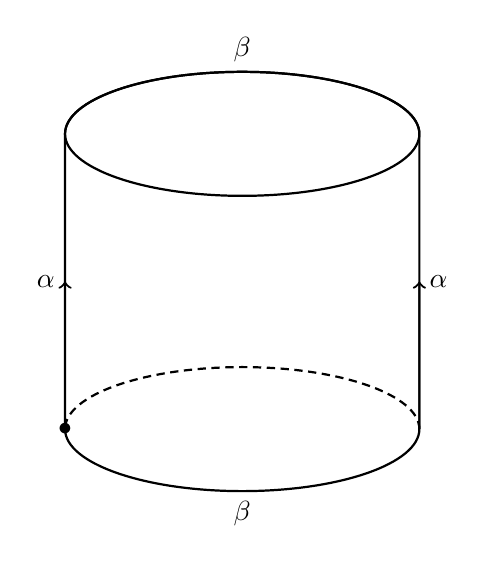
\begin{tikzpicture}[scale = 3]
			\draw [thick]
  				(180:7.5mm) coordinate (A)
				-- ++(0,-12.5mm) coordinate [midway] (E) coordinate (B) node [midway,left] {$\alpha$}
				arc (180:360:7.5mm and 2.625mm) coordinate (D) node [midway,below] {$\beta$}
				-- (A -| D) coordinate [midway] (F) coordinate (C) node [midway,right] {$\alpha$} arc (0:180:7.5mm and 2.625mm) node [midway,above] {$\beta$};
  			\draw [thick]
  				(0,0) coordinate (T) circle (7.5mm and 2.625mm);
  			\draw [thick,densely dashed] (D) arc (0:180:7.5mm and 2.625mm);
			\draw [thick,->] (B) -- (E);
			\draw [thick,->] (D) -- (F);
			\path [] (A) -- (C) node [midway] {$\circlearrowleft$};
			\path [] (B) -- (D) node [midway] {$\circlearrowleft$};
			\node at (B) {$\bullet$};
		\end{tikzpicture}
		\caption{$n > 1$.}
		\label{fig:n>1}
	\end{subfigure}
	\caption{Whitehead bracket and the conjugation action.}
	\label{fig:conjugation_action}
\end{figure}

\begin{figure}[h!tb]
	\centering
	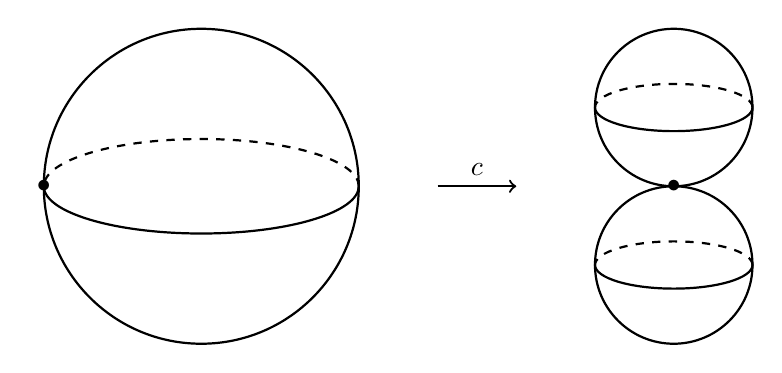
\begin{tikzpicture}
	\draw [->,thick] (0,0) -- (1,0) node[midway,above] {$c$};
		\draw[thick] (-3,0) circle (2cm);
		\draw[thick] (-5,0) arc (180:360:2 and 0.6);
  		\draw[dashed,thick] (-1,0) arc (0:180:2 and 0.6);
		\node at (-5,0) {$\bullet$};
		\draw[thick] (3,1) circle (1cm);
		\draw[thick] (2,1) arc (180:360:1 and 0.3);
  		\draw[dashed,thick] (4,1) arc (0:180:1 and 0.3);
		\draw[thick] (3,-1) circle (1cm);
		\draw[thick] (2,-1) arc (180:360:1 and 0.3);
  		\draw[dashed,thick] (4,-1) arc (0:180:1 and 0.3);
		\node at (3,0) {$\bullet$};
	\end{tikzpicture}
	\caption{The collapsing map $c : \mathbb{S}^n \to \mathbb{S}^n \vee \mathbb{S}^n$.}
	\label{fig:collapsing_map}
\end{figure}

\section{Grading}
Let $(X,p) \in \mathsf{Top}_\ast$. For $n \in \omega$ let $L^n := \pi_{n + 1}(X,p)$ and define
\begin{equation*}
	L := \bigoplus_{n \in \omega} L^n.
\end{equation*}
Moreover, define $[-,-] : L \times L \to L$ by
\begin{equation*}
	\sbr[3]{\sum_i \alpha_i, \sum_j \beta_j} := \sum_{i,j} [\alpha_i,\beta_j].
\end{equation*}
Then clearly $L^nL^m \subseteq L^{n + m}$ holds. It also turns out, that we have a Lie algebra-like structure on $L$, i.e. the bracket is bilinear, alternating and there is a Jacobi identity (for more details see \cite[474--478]{whitehead:homotopy_theory:1978}). 

\begin{proposition}
	Let $n,m \in \omega$, $n \geq 1$, $[\alpha_1], [\alpha_2] \in \pi_{n + 1}(X)$ and $[\beta] \in \pi_{m + 1}(X)$. Then
	\begin{equation*}
		[\alpha_1 + \alpha_2, \beta] = [\alpha_1,\beta] + [\alpha_2,\beta] \qquad \text{and} \qquad [\beta,\alpha_1 + \alpha_2] = [\beta,\alpha_1] + [\beta,\alpha_2].
	\end{equation*}
\end{proposition}

Recall, that for $n \geq 1$ we have that $H_n(\mathbb{S}^n) \cong \mathbb{Z}$. Thus if we are given any continuous map $f : \mathbb{S}^n \to \mathbb{S}^n$, the induced map $H_n(f)$ is simply a multiplication by a unique integer. This integer is defined to be the \bld{degree of $f$}, written $\deg f$. Observe that lemma \ref{lem:order_reversing} stays true if we consider a homeomorphism $h : (\mathbb{S}^n,\ast) \to (\mathbb{S}^n,\ast)$ with $\deg h = -1$. Indeed, this basically follows from the relative homeomorphism theorem which states that
\begin{equation*}
	H_k(q) : H_k(\mathbb{D}^n,\mathbb{S}^{n - 1}) \to H_k(\mathbb{S}^n,\ast) \cong \wtilde{H}_k(\mathbb{S}^k)
\end{equation*}
\noindent is an isomorphism for all $k \in \omega$.

\begin{proposition}
	\label{prop:graded_commutative}
	Let $n,m \in \omega$, $[\alpha] \in \pi_{n + 1}(X)$ and $[\beta] \in \pi_{m + 1}(X)$. Then
	\begin{equation*}
		[\beta,\alpha] = (-1)^{(n + 1)(m + 1)}[\alpha,\beta].
	\end{equation*}
\end{proposition}

\begin{proof}
	Consider the \bld{permutation map} $\sigma : \mathbb{S}^{n + m + 1} \to \mathbb{S}^{n + m + 1}$ defined by
	\begin{equation*}
		(y_1,\dots,y_{m + 1},x_1,\dots,x_{n + 1}) \mapsto (x_1, \dots,x_{n + 1},y_1,\dots,y_{m + 1}).
	\end{equation*}
	Then clearly $\deg \sigma = (-1)^{(n + 1)(m + 1)}$, since $\sigma$ is the composition of permutations and hence orthogonal transformations. An application of lemma \ref{lem:order_reversing} yields 
	\begin{equation*}
		[\beta,\alpha] = [(\beta \vee \alpha) \circ f] = [(\alpha \vee \beta) \circ f \circ \sigma] = (-1)^{(n + 1)(m + 1)}[\alpha,\beta].
	\end{equation*}
\end{proof}

\begin{proposition}
	Let $n,m,r \in \omega$, $n,m,r \geq 1$, $[\alpha] \in \pi_{n + 1}(X)$, $[\beta] \in \pi_{m + 1}(X)$ and $[\gamma] \in \pi_{r + 1}(X)$. Then
	\begin{equation*}
		(-1)^{r(n + 1)}[\alpha,[\beta,\gamma]] + (-1)^{n(m + 1)}[\beta,[\gamma,\alpha]] + (-1)^{m(r + 1)}[\gamma,[\alpha,\beta]] = 0
	\end{equation*}
\end{proposition}

\printbibliography
\end{document}
